\documentclass[20pt,,margin=1in,innermargin=-4.5in,blockverticalspace=-0.25in]{tikzposter}
\geometry{paperwidth=43in,paperheight=32.5in}
\usepackage[utf8]{inputenc}
\usepackage{amsmath}
\usepackage{amsfonts}
\usepackage{amsthm}
\usepackage{amssymb}
\usepackage{mathrsfs}
\usepackage{graphicx}
\usepackage{adjustbox}
\usepackage{enumitem}
\usepackage{wrapfig}
\usepackage{SUtheme}
\usepackage{comment}
\usepackage{mwe} % for placeholder images
\usepackage{tikz}
% set theme parameters
\tikzposterlatexaffectionproofoff
\usetheme{SUTheme}
\usecolorstyle{SUStyle}
\usetitlestyle{Filled}

\usepackage[scaled]{helvet}
\renewcommand\familydefault{\sfdefault}
\usepackage[T1]{fontenc}


\title{A Symmetry Problem}
\author{Ethan Martirosyan and Yingpeng He \, Mentor: Jihye Lee}
\institute{University of California Santa Barbara}
\titlegraphic{\includegraphics[width=0.06\textwidth]{logo.png}}

% begin document
\begin{document}
\maketitle
\centering

\begin{columns}
    \column{0.32}
    \block{Introduction}{
                  Let us consider the following problem. Let $\Omega \subseteq \mathbb{R}^n$ be a domain that is bounded, open, and connected. Furthermore, suppose that the boundary $\partial{\Omega}$ is smooth. Let $u: \Omega \rightarrow \mathbb{R}$ be a $C^2$ function that satisfies the following conditions: $\Delta u = -1$ in $\Omega$ and $u=0$ and $\frac{\partial{u}}{\partial{n}} = c$ on $\partial{\Omega}$ for some constant $c$. Then, $\Omega$ must be a ball. Furthermore, we know that $u(x) = (b^2-r^2)/2n$, where $b$ is the ball's radius and $r$ is the distance to its center.
    }
    \block{First Proof}{
     The first proof we present is from Professor James Serrin [3].
    This proof utilizes the moving plane method. Let $T_0$ be a $n-1$ dimensional hyperplane in $\mathbb{R}^n$ that does not intersect the domain $\Omega$. We begin to move this plane normal to itself until it intersects $\Omega$. When this occurs, the new plane $T$ splits $\Omega$ into two parts. The part of $\Omega$ that lies on the same side of $T$ as our initial plane $T_0$ is denoted by $\Sigma(T)$. We reflect $\Sigma(T)$ in $T$ to obtain $\Sigma^\prime := \Sigma^\prime(T)$. As $T$ moves through $\Omega$, $\Sigma^\prime$ will remain in $\Omega$ until it becomes internally tangent to $\Omega$ at a point $P$ or $T$ becomes orthogonal to $\Omega$ at some point $Q$. When either of these occurs, we stop moving the plane $T$, and we denote the resulting plane by $T^\prime$. We claim that $\Omega$ is symmetric about $T^\prime$. Showing this would prove the theorem. To see how, we recall that the plane $T_0$ was chosen arbitrarily. If $\Omega$ is symmetric about $T^\prime$, then $\Omega$ is symmetric in all possible directions. Since $\Omega$ is simply connected and has this strong symmetry property, it must be a ball.   
\\
\\
\begin{center}


\tikzset{every picture/.style={line width=0.75pt}} %set default line width to 0.75pt        

\begin{tikzpicture}[x=0.75pt,y=0.75pt,yscale=-1.65,xscale=1.65]
%uncomment if require: \path (0,571); %set diagram left start at 0, and has height of 571

%Shape: Polygon Curved [id:ds5706838743203553] 
\draw   (45,134) .. controls (125,120) and (96,266) .. (131,271) .. controls (166,276) and (189.5,110) .. (245.5,149) .. controls (301.5,188) and (165,468) .. (127,467) .. controls (89,466) and (-35,148) .. (45,134) -- cycle ;
%Straight Lines [id:da32245607071165727] 
\draw    (20.5,366) -- (253.5,365) ;
%Shape: Polygon Curved [id:ds09219005382763679] 
\draw   (131,271) .. controls (148,271) and (202.13,366.75) .. (201.5,366) .. controls (200.88,365.25) and (68,366.75) .. (63.88,366) .. controls (59.75,365.25) and (114,271) .. (131,271) -- cycle ;
%Straight Lines [id:da8205571992315139] 
\draw    (21.5,491) -- (259.5,491) ;
%Shape: Polygon Curved [id:ds6503069563047057] 
\draw   (497.5,135) .. controls (520.5,136) and (581.5,203) .. (607.5,256) .. controls (633.5,309) and (553.5,517) .. (496.5,517) .. controls (439.5,517) and (369,311) .. (373.5,261) .. controls (378,211) and (474.5,134) .. (497.5,135) -- cycle ;
%Straight Lines [id:da32516902000919035] 
\draw    (337.5,271) -- (633.5,273) ;
%Straight Lines [id:da6980504582735876] 
\draw    (333,106) -- (629,109) ;
%Shape: Polygon Curved [id:ds3409580382825572] 
\draw   (374.5,271) .. controls (384.5,273) and (595.5,272) .. (610.5,272) .. controls (625.5,272) and (554.5,408) .. (498.5,410) .. controls (442.5,412) and (364.5,269) .. (374.5,271) -- cycle ;
%Straight Lines [id:da22457687318989672] 
\draw    (205.13,487.5) -- (204.89,457.5) ;
\draw [shift={(204.88,455.5)}, rotate = 89.55] [color={rgb, 255:red, 0; green, 0; blue, 0 }  ][line width=0.75]    (10.93,-3.29) .. controls (6.95,-1.4) and (3.31,-0.3) .. (0,0) .. controls (3.31,0.3) and (6.95,1.4) .. (10.93,3.29)   ;
%Straight Lines [id:da3600925863165976] 
\draw    (369.13,112) -- (368.9,133.5) ;
\draw [shift={(368.88,135.5)}, rotate = 270.61] [color={rgb, 255:red, 0; green, 0; blue, 0 }  ][line width=0.75]    (10.93,-3.29) .. controls (6.95,-1.4) and (3.31,-0.3) .. (0,0) .. controls (3.31,0.3) and (6.95,1.4) .. (10.93,3.29)   ;

% Text Node
\draw (273,483.4) node [anchor=north west][inner sep=0.75pt]    {$T_{0}$};
% Text Node
\draw (269,355.4) node [anchor=north west][inner sep=0.75pt]    {$T^{\prime }$};
% Text Node
\draw (130,241.4) node [anchor=north west][inner sep=0.75pt]    {$P$};
% Text Node
\draw (126,315.4) node [anchor=north west][inner sep=0.75pt]    {$\Sigma ^{\prime }$};
% Text Node
\draw (109,393.4) node [anchor=north west][inner sep=0.75pt]    {$\Sigma \left( T^{\prime }\right)$};
% Text Node
\draw (58,211.4) node [anchor=north west][inner sep=0.75pt]    {$\Omega $};
% Text Node
\draw (620,238.4) node [anchor=north west][inner sep=0.75pt]    {$Q$};
% Text Node
\draw (313,262.4) node [anchor=north west][inner sep=0.75pt]    {$T^{\prime }$};
% Text Node
\draw (305,98.4) node [anchor=north west][inner sep=0.75pt]    {$T_{0}$};
% Text Node
\draw (487,313.4) node [anchor=north west][inner sep=0.75pt]    {$\Sigma ^{\prime }$};
% Text Node
\draw (477,207.4) node [anchor=north west][inner sep=0.75pt]    {$\Sigma \left( T^{\prime }\right)$};
% Text Node
\draw (493,440.4) node [anchor=north west][inner sep=0.75pt]    {$\Omega $};


\end{tikzpicture}
\end{center}
    To prove this, we introduce the function $v: \Sigma^\prime \rightarrow \mathbb{R}$ defined by $v(x) = u(x^\prime)$ for $x \in \Sigma^\prime$, where $x^\prime$ is the reflection of $x$ across $T^\prime$. By the maximum principle, we deduce that $u - v > 0$ or $u-v = 0$ in $\Sigma^\prime$. For the sake of contradiction, suppose that $u-v > 0$.  If $\Sigma^\prime$ is internally tangent to $\Omega$ at some point $P$, then we may appeal to the boundary point maximum principle to deduce that $\frac{\partial}{\partial{n}}(u-v) > 0$ at $P$ [1]. However, we know that $\partial{u}/\partial{n} = \partial{v}/\partial{n} = c$. Thus we have reached a contradiction. If $T^\prime$ is orthogonal to the boundary of $\Omega$ at some point $Q$, then we show that $u$ and $v$ have the same first and second derivatives at $Q$. Using a modified version of the boundary point maximum principle, we can also show that $\frac{\partial}{\partial{s}} (u-v) > 0 \text{ or } \frac{\partial^2}{\partial^2{s}}(u-v) > 0$ for any direction $s$ that enters $\Sigma^\prime$ non-tangentially at $Q$. However, this directly contradicts the fact that $u$ and $v$ have the same first and second derivatives at $Q$. We may thus conclude that $\Omega$ is symmetric about $T^\prime$.
}


    \column{0.36}
    \block{Second Proof}{
        The second proof we present is from Weinberger [2]. To start, we first compute
\[
\Delta\bigg(r \frac{\partial{u}}{\partial{r}}\bigg) = r \frac{\partial}{\partial{r}} (\Delta u) + 2\Delta = -2
\] where $r$ is the distance to the origin. Using this and the fact that $\Delta u = -1$, we obtain
\[
\int_\Omega \bigg[ 2u - r\frac{\partial{u}}{\partial{r}}\bigg] dx = \int_\Omega \bigg[ -u \Delta \bigg(r \frac{\partial{u}}{\partial{r}} \bigg) + r \frac{\partial{u}}{\partial{r}} \Delta u \bigg] dx
\]
    Using Green's identity yields
\[
\int_\Omega \bigg[ -u \Delta \bigg(r \frac{\partial{u}}{\partial{r}} \bigg) + r \frac{\partial{u}}{\partial{r}} \Delta u \bigg] dx = \int_{\partial{\Omega}} \bigg[ - u \frac{\partial}{\partial{n}}\bigg(r\frac{\partial{u}}{\partial{r}}\bigg)+ r \frac{\partial{u}}{\partial{r}}\frac{\partial{u}}{\partial{n}}\bigg] dS
\] By assumption, we have $u = 0$ on $\partial{\Omega}$. Thus, we find that
\[
\int_{\partial{\Omega}} \bigg[ - u \frac{\partial}{\partial{n}}\bigg(r\frac{\partial{u}}{\partial{r}}\bigg)+ r \frac{\partial{u}}{\partial{r}}\frac{\partial{u}}{\partial{n}}\bigg] dS =  \int_{\partial{\Omega}} r \frac{\partial{r}}{\partial{n}} \bigg(\frac{\partial{u}}{\partial{n}}\bigg)^2 dS
\] By assumption, we know that $\partial{u}/\partial{n} = c$ on $\partial{\Omega}$. Thus, we find that
\[
\int_{\partial{\Omega}} r \frac{\partial{r}}{\partial{n}} \bigg(\frac{\partial{u}}{\partial{n}}\bigg)^2 dS = c^2 \int_{\partial{\Omega}} r\frac{\partial{r}}{\partial{n}} dS = c^2 n \int_{\Omega} dx =  nc^2 V
\] Green's theorem also implies
\[
\int_{\Omega} r \frac{\partial{u}}{\partial{r}} dx = -n \int_{\Omega} u dx
\] so that substitution yields
\[
(n+2) \int_\Omega u d x = nc^2V
\] However, we also note that
\[
1 = (\Delta u)^2 \leq n \sum_{i=1}^n u_{ii}^2 \leq n \sum_{i,j} u_{ij}^2
\] by the Cauchy-Schwarz inequality. From this, we deduce that
\[
\Delta\bigg( \vert \nabla u\vert^2 + \frac{2}{n}u\bigg) = 2\sum_{i,j} u_{ij}^2 - \frac{2}{n} \geq 0
\] Using this and the fact that $\vert \nabla u \vert^2 + (2/n)u = c^2$ on $\partial{\Omega}$, we may appeal to the maximum principle to deduce that $\vert \nabla u \vert + (2/n)u < c^2$ in $\Omega$ or $\vert \nabla u \vert + (2/n)u = c^2$ in $\Omega$. If the former inequality held, then we could integrate over $\Omega$ to deduce that
\[
(n+2)\int_\Omega u dx < nc^2V
\] This contradiction informs us that $\vert \nabla u \vert^2 + (2/n)u = c^2$ in $\Omega$ so that
\[
\Delta\bigg( \vert \nabla u\vert^2 + \frac{2}{n}u\bigg) = 2\sum_{i,j} u_{ij}^2 - \frac{2}{n} = 0
\]
and
\[
1 = n \sum_{i=1}^n u_{ii}^2 = \sum_{i,j} u_{ij}^2
\] which implies that $u_{ij} = -\delta_{ij}/n$. Solving the corresponding partial differential equations yields
\[
u = \frac{1}{2n}(B - r^2)
\] where $B$ is a constant. Since $u = 0$ on $\partial{\Omega}$, $B$ is positive and $\Omega$ is a ball of radius $B^{1/2}$.

    }

    \column{0.32}
    \block{Applications}{
       This theorem is significant because it allows us to determine the shape of $\Omega$ from properties of $u$. It also has many applications in physics. For example, we may consider an incompressible viscous fluid moving through a straight pipe of cross sectional form $\Omega$. If we fix a rectangular coordinate system with the $z$-axis directed along the pipe, then the velocity $u$ depends only on $x$ and $y$, and it satisfies the differential equation $\Delta u = -A$ for some constant $A$. Furthermore, because the fluid is viscous, we know that $u = 0$ on $\partial{\Omega}$; that is, there is no movement on the boundary of the pipe. Finally, we note that $\mu\partial{u}/\partial{n}$ is the tangential stress on the pipe wall, where $\mu$ is the viscosity constant. If the tangential stress is constant, then we may apply the above theorem to conclude that $\Omega$ is a circular cross section.
    }
    \block{Further Results}{
    There is an interesting extension of this theorem from Wolfgang Reichel [4]. Let $\Omega_0$ and $\Omega_1$ be smooth domains and let $\Omega = \Omega_0 \setminus \overline{\Omega}_1$ be connected. Suppose that $f \in C^1$ is a function satisfying $\Delta u + f(u, \vert \nabla u\vert) = 0$ in $\Omega$, $0 < u < a$ in $\Omega$, $u = 0$ on $\partial{\Omega_0}$, $u = a$ on $\partial{\Omega_1}$, and $\partial{u}/{\partial{n}} = c_i$ on $\Omega_i$. Then, we conclude that $\Omega$ is an annulus and $u$ is radially symmetric and decreasing in $r$.
    
\begin{center}


\tikzset{every picture/.style={line width=0.75pt}} %set default line width to 0.75pt        

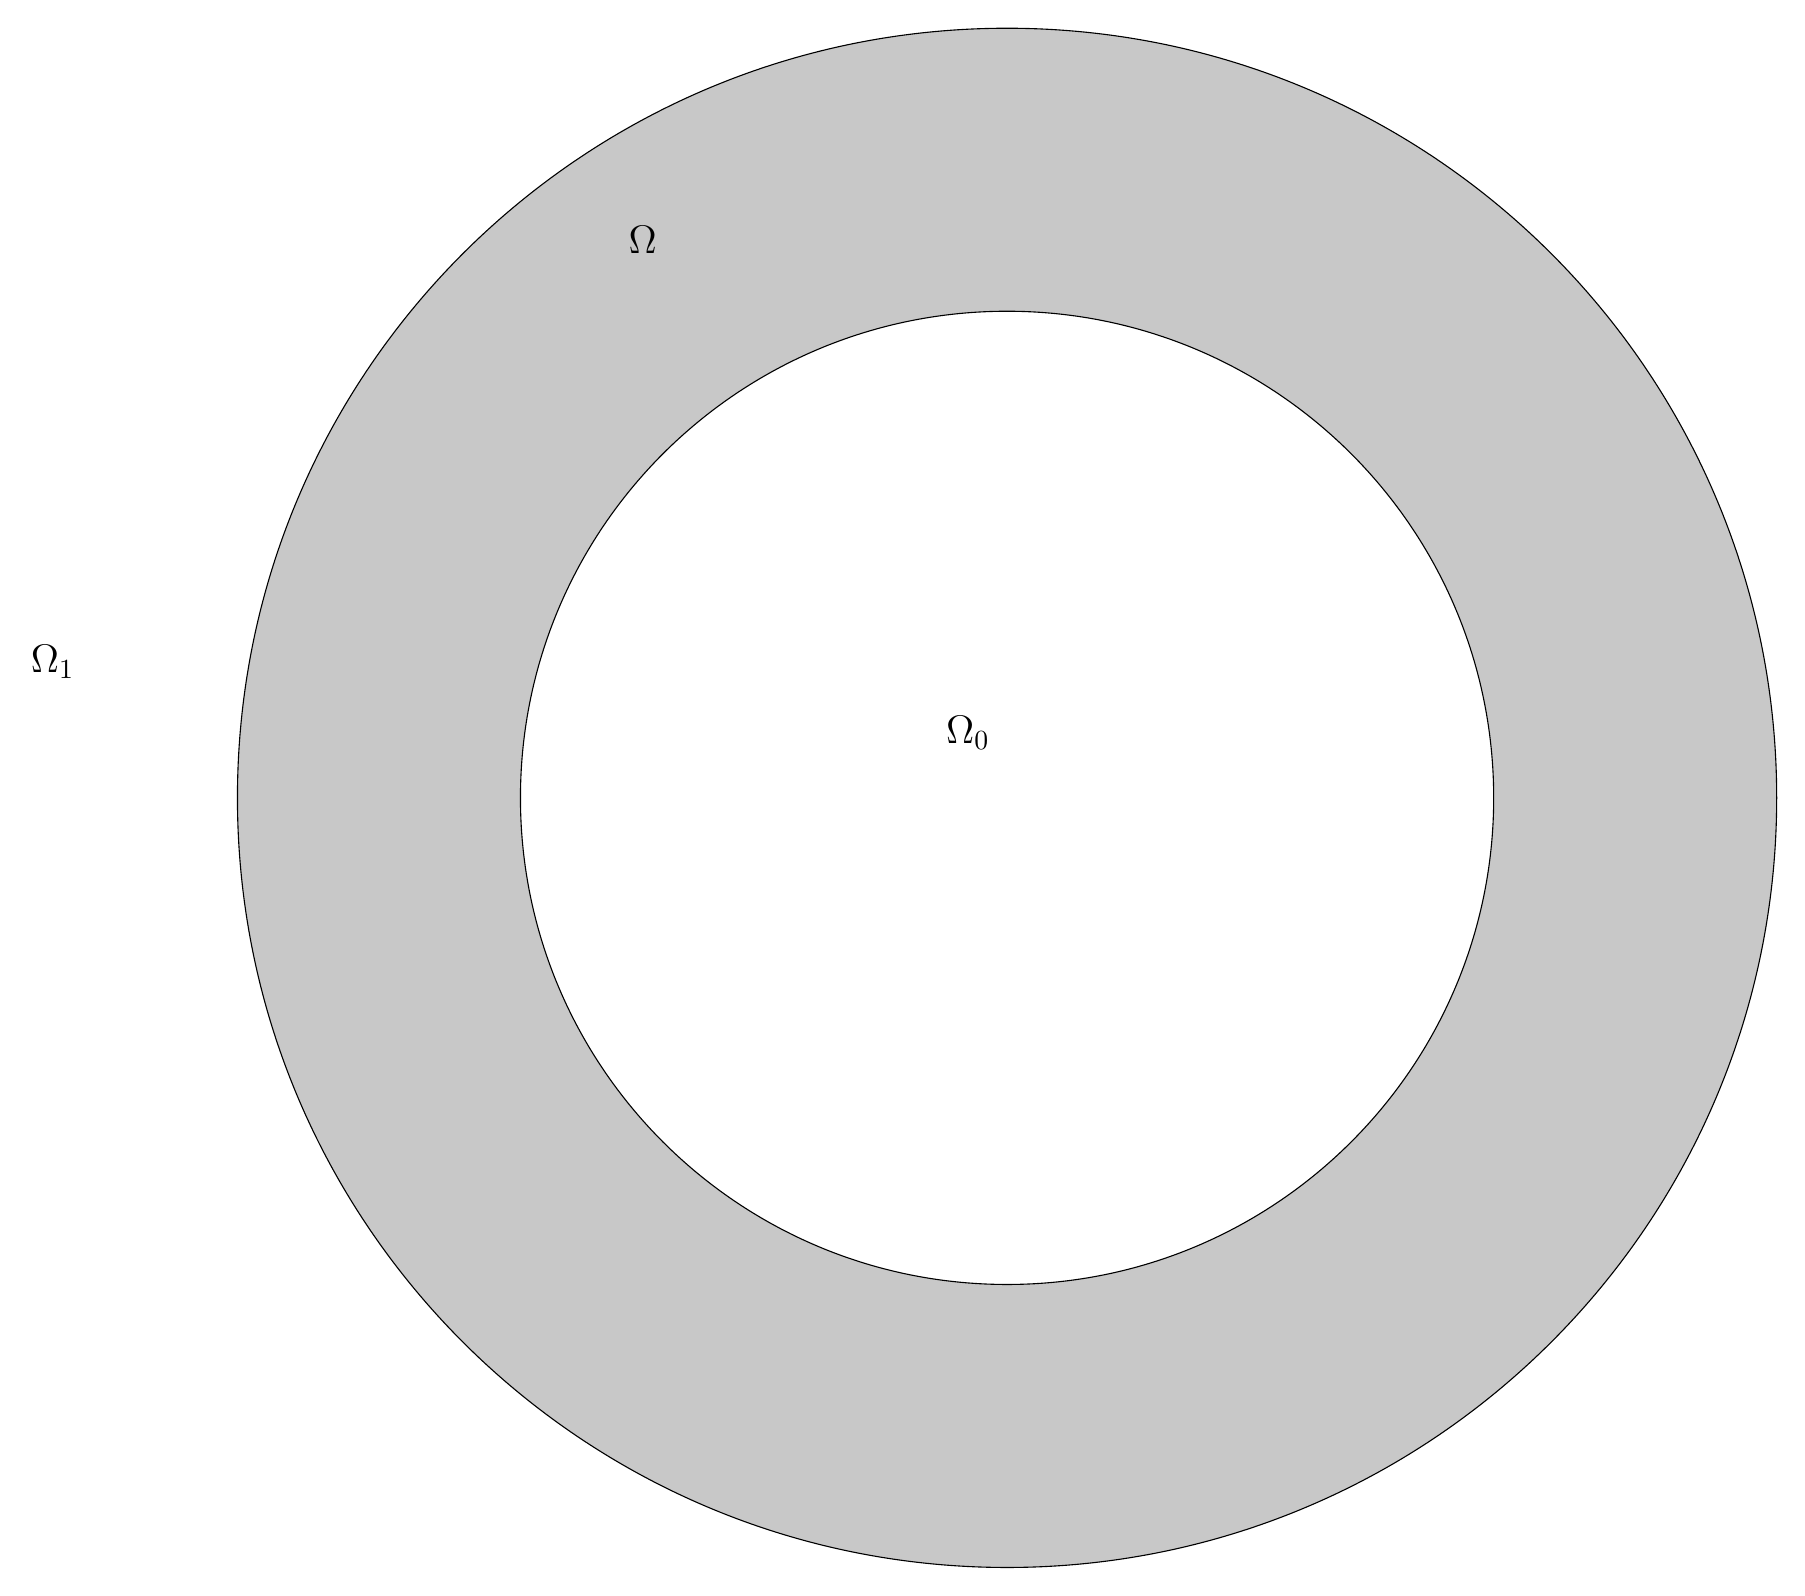
\begin{tikzpicture}[x=0.75pt,y=0.75pt,yscale=-1.8,xscale=1.8]
%uncomment if require: \path (0,472); %set diagram left start at 0, and has height of 472

%Shape: Circle [id:dp8921067574796464] 
\draw  [color={rgb, 255:red, 0; green, 0; blue, 0 }  ,draw opacity=1 ][fill={rgb, 255:red, 200; green, 200; blue, 200 }  ,fill opacity=1 ] (127,235) .. controls (127,121.23) and (219.23,29) .. (333,29) .. controls (446.77,29) and (539,121.23) .. (539,235) .. controls (539,348.77) and (446.77,441) .. (333,441) .. controls (219.23,441) and (127,348.77) .. (127,235) -- cycle ;
%Shape: Circle [id:dp12450006417670667] 
\draw  [fill={rgb, 255:red, 255; green, 255; blue, 255 }  ,fill opacity=1 ] (202.75,235) .. controls (202.75,163.06) and (261.06,104.75) .. (333,104.75) .. controls (404.94,104.75) and (463.25,163.06) .. (463.25,235) .. controls (463.25,306.94) and (404.94,365.25) .. (333,365.25) .. controls (261.06,365.25) and (202.75,306.94) .. (202.75,235) -- cycle ;

% Text Node
\draw (316,212.4) node [anchor=north west][inner sep=0.75pt]  [font=\Large]  {$\Omega _{0}$};
% Text Node
\draw (231,81.4) node [anchor=north west][inner sep=0.75pt]  [font=\Large]  {$\Omega $};
% Text Node
\draw (71,193.4) node [anchor=north west][inner sep=0.75pt]  [font=\Large]  {$\Omega _{1}$};


\end{tikzpicture}
\end{center}
    }    
    \block{Acknowledgements}{
    We would like to thank Jihye Lee for mentoring us. Furthermore, we express gratitude to the 2024 UCSB Directed Reading Program for giving us this opportunity.
    }
   
    \block{References}{
    \footnotesize
   
[1] Hans Weingberger. Maximum Principles in Differential Equations. 1984.

[2] Hans Weingberger. Remark on the Preceding Paper of Serrin. \emph{Arch. Rational Mech. Anal.} 1971.

[3] James Serrin. A Symmetry Problem in Potential Theory. \emph{Arch. Rational Mech. Anal.} 1971.

[4] Wolfgang Reichel. Radial Symmetry for Elliptic Boundary-Value Problems on Exterior Domains. \emph{Arch. Rational Mech. Anal.} 1997.


    }
\end{columns}
\end{document}